\documentclass[11pt,a4paper]{article}
\setlength{\parindent}{0ex}
\setlength{\parskip}{1em plus1ex minus.5ex}
%% $Id$
\usepackage{fullpage}
\usepackage{verbatim}
\usepackage[dvips]{graphicx}
%%\addtolength{\textheight}{2cm}
\begin{document}

\pagestyle{empty}

\begin{titlepage}
  \begin{center}
    \Huge
    \textbf{Apache Tcl}

    \sffamily
    \small
    Fast, Light, Easy, Powerful\\

    By David N. Welton, Apache Software Foundation\\

    \footnotesize
    davidw@apache.org
    \normalsize
  \end{center}
\end{titlepage}

\sffamily

\begin{abstract}
  Programming for the web can be both easy and powerful, quick and
  elegant, fast, and lightweight.  Find out about what's available for
  both new users and experienced programmers, as we cover everything
  from how to get started, different systems available, programming
  strategies, and the low-level beauty of integrating Apache and Tcl.
\end{abstract}

\tableofcontents

\section{Introduction to Apache and Tcl}

\subsection{Apache}

Apache Tcl is, of course, the name for the projects which have the
Apache web server and Tcl language in common, but more than that, we
have all arrived at this junction between Apache and Tcl because we
have found it to be the optimal solution.

Apache is, of course, the world's most popular web server.  According
to netcraft, Apache accounts for around 60\% of the web server market,
putting it ahead of all other contenders combined.

Apache is very flexible, fast, correct and secure. To attach meanings
to these descriptions, let's go through them and explain.

The flexibility in Apache lies in its ability to be configured in many
different ways, from minimalistic to a full-fledged ``web
application'' server.

While there are faster web servers available, Apache competes very
admirably with the current offerings on the market.

Of great importance, Apache is correct - it adheres to defined
Internet standards.

And, most of all, Apache is very secure.  The code has been examined
by experts the world over, and when bugs are discovered, fixes are
promptly available.

The Apache web server was first created by a group of sysadmins who
were using the NCSA server and had created patches to enhance and
improve it. Thus, "A Patchy" web server.

The Apache Software Foundation now encompasses a large variety of
diverse projects in addition to Tcl: the web server, XML, Java, Perl,
PHP, APR, Python, and is a non-profit corporation registered in the
U.S., with members throughout the world.

The ASF consists of 60-some members, and hundreds of "committers" -
those who have the rights to make changes to different projects' code.

\subsection{Tcl}

Tcl stands for ``Tool Command Language''. It was created in the late
80'ies, by John Ousterhout, then a professor at the University of
California at Berkeley, as a replacement for the many small extension
languages he was writing for his applications. From the very
beginning, Tcl was engineered to be combined with other systems.

The original idea behind Tcl is still very valid today: powerful
applications can be made much more so by letting the user access parts
of them programmatically. One-off languages are best replaced by a
more general solution. The answer: a reusable library that provides a
scripting language.  This allows for ``embedding and extending'' of
Tcl.  It can either be ``embedded'' into another application, where
the other program controls what is going on, and calls Tcl, or
``extended'', which means that Tcl is in control, and it either has
extra code built in, or it loads it dynamically.  Apache Tcl projects
are almost exclusively of the first type.  Apache is the center of
attention, and it makes calls to Tcl at opportune times.

Let's look at some of Tcl's most important features:

First of all, it's easy to learn, having a very simple syntax.  This
means that anyone can pick it up and start using it almost right away,
even if they are not an expert software engineer.  As we will see
later, this is at times important for a web language.

Despite being easy, Tcl is also quite flexible.  It doesn't limit the
expert programmer, and encourages them to take advantage of its
features in order to solve problems most elegantly.  It is actually
possible to create new control structures such as 'if' or 'while' in
Tcl code itself, without resorting to C!

As mentioned above, embedding and extending are central to Tcl's
philosophy.  It is possible to access a great deal of the language's
internals via its well-documented C API.

What's more, Tcl doesn't take up up a lot of system resources.  It
doesn't waste memory, nor disk space, and is reasonably fast as a
byte-compiled scripting language.

Of course, Tcl is Free Software.  You can do pretty much anything you
like with it, as it's distributed under the very liberal BSD-style
license.  It's used in many free software projects, as well as
proprietary applications in large corporations.

Another point that needs mentioning is that the Tcl language is
natively multiplatform.  It is designed to work equally well on Unix,
Windows, as well as both Mac OS classic and MacOS X.

The Tk toolkit is almost always mentioned in the same phrase as Tcl,
but it's important to understand that they are two separate things,
despite both being developed by John Ousterhout, and having a closely
entwined history.  Tk is a graphical toolkit for rapidly developing
visual applications with a native look and feel.

Not only does Tcl do the simple things well, it also makes complex
things possible (to borrow a phrase).  The standard library, tcllib,
contains code to perform all kinds of tasks, as well as manage complex
data structures, such as graphs, queues, matrixes, etc...  As a
testament to Tcl's flexibility, not even object orientation is built
into the language itself, but can be loaded as a package, the most
popular one being [Incr Tcl].  Tcl has been around long enough that
there is probably a package out there that does what you need.

\subsection{Tcl and the Web}

The web (and XML, for that matter) is primarily text oriented, so a
language that's good at dealing with text is well suited to the web,
and much, much faster to develop with than a low-level language like
C.  This is why languages like Perl and Tcl have been so successful
for web programming to date.  It's easier, security is improved by not
worrying about buffer overflows, and everything is generally more
flexible.

The second big advantage when using a ``scripting language'' for the
web is that it makes the craft of creating dynamic web pages available
to more people, who might not necessarily be skilled enough to use a
more complex language such as Java or C++.  Not everyone who needs to
get something up on the web has the luxury of knowing many languages,
and/or having the time to learn a more difficult one.  While Tcl is a
fine tool in the hands of an expert software engineer, it is also
particularly well suited to this type of use, because of its simple
structure, and the ease with which it is learned.  As an added bonus,
having learned the language, it can be used beyond the web for system
tasks, graphical apps, and more.

As far back as 1995, when many of us were still experimenting with
simplistic CGI's, Tcl was being integrated into what was to go on to
become Vignette's StoryServer, and AOLserver, two systems that are
still in use today.  AOLserver is even open source, and is a very well
regarded high-performance, multi-threaded web server with built-in
scriptability, thanks to Tcl.

\subsection{Tcl Example 1.}

A few small examples of Tcl code follow.  They demonstrate some of the
fundamental constructs of the language.

\begin{verbatim}
set seconds [clock seconds]
puts "The time is [clock format \$seconds]"
\end{verbatim}

In the above example, 3 Tcl commands are used, ``set'', ``puts'', and
``clock''.  The first line sets the variable ``seconds'' to the value
returned by the command ``clock seconds''.  In the second line,
``clock format'' is called with the variable \$seconds and the result
is left inside the string which is then passed to ``puts'', which will
send it to stdout.

\begin{verbatim}
proc greeting {lang} {
    switch \$lang {
        en {
            return "Hello, how is it going?"
        }
        it {
            return "Buon giorno, come va?"
        }
        fr {
            return "Bonjour, .......?"
        }
        de {
            return "Guten Tag, wie gehts?"
        }
        zt {
            return "Gr�ezi, wi gaat's?"
        }
    }
}
\end{verbatim}

This is an example of a ``proc'' - a new Tcl procedure or command.  It
accepts one argument, ``lang'', which it then proceeds to examine, and
then return a different string depending on the result.

\section{Apache Tcl}

Our projects aren't just related by the fact that we all use Tcl - the
Apache Tcl projects share a common philosophy that "simple things
should be easy, and hard things should be possible" (to borrow a quote
- it works well for them!). We all arrived at Tcl not because it's the
only tool in our box, but because for us it is the right tool.

The "Apache Tcl Project" is currently comprised of 5 individual
projects, and is moving towards having 3, or less, in the future.

\includegraphics[scale=0.6]{./future.ps}

Getting ahead of ourselves, our short term plans are to release Rivet,
and phase out mod\_dtcl and NeoWebScript.  Long term, if possible, we
will further modularize all our offerings, so that at some point, it
would be possible to run Rivet and Websh as loaded packages from
within mod\_tcl, as it is capable of giving us low level access to the
Apache internals from Tcl.  So, we wouldn't really only have one
project, but there would be, at the same time, more modularity and
tighter integration amongst the remaining systems.

Without further ado, our 5 projects are:

\begin{itemize}
\item mod\_dtcl\\
  mod\_dtcl was created in 1998 by David Welton, and, while there were
  other products out there that did similar things, mod\_dtcl was one
  of the first that was Free Software.

  The Apache Software Foundation subsequently created the Tcl group,
  with mod\_dtcl as its basis in late 2000.

  mod\_dtcl will eventually be replaced by Apache Rivet, which is
  infact, getting just about 100\% of our development time lately.

  The original design goals of mod\_dtcl were based on observations
  about the success of PHP, and sought to borrow the best of that
  system, while avoiding some of the downfalls.  Principally, mod\_dtcl
  was meant to be fast, light, and simple to use.

\item NeoWebScript\\
  NeoWebScript was created by Karl Lehenbauer, one of the early Tcl
  users and contributors and is currently maintained by Damon
  Courtney. NWS, as it's known, became part of the Apache Tcl project
  in early 2001, after having been released as Free Software.  In its
  early years, NWS was not really ``Open Source''.

  NWS was written with an ISP type environment in mind, and as a
  consequence, as features such as a sandbox, utilizing Tcl's safe
  interpreters, which is able to keep users contained.  In addition,
  NWS aims to make a lot of popular extensions such as 'gd' and
  database extensions available as part of the core product.

\item mod\_tcl\\
  mod\_tcl was created by Michael Link, for Apache 2.0, with the goal
  of exposing the Apache API in Tcl, in order to make it possible to
  write Apache modules in Tcl.  Most of the other projects take
  advantage of Apache features, and are tightly linked to the server,
  but could conceivably also independent of Apache.  mod\_tcl takes
  the opposite approach and gives you access to a great deal of
  Apache's C API.  This flexibility means that, one day, other Apache
  Tcl modules might conceivably just be plugins for mod\_tcl.

\item Websh\\
  Websh was born in 1995 as a C++ library incorporating a Tcl
  interpreter, and gradually migrated to being a Tcl extension. It
  became Free Software in 2000, and was contributed to the ASF in
  2001. Andrej Vckovski was the original author, with major work done
  by Ronnie Brunner (Websh 2) and Simon Hefti (Websh 3).

  Websh is more of a complete ``application development'' environment
  than the other systems, which is in some ways a tradeoff.  It
  provides many powerful tools for the programmer, but takes more time
  to learn, and requires just a bit more ramp-up time to start
  creating pages.

  One unique feature of Websh is that it is relatively independent of
  Apache, and, infact, version is provided that runs as a stand-alone
  CGI.

\item Apache Rivet\\
  The most recent of the Apache Tcl projects, Rivet is the future of
  both mod\_dtcl and NeoWebScript.  Both David Welton and Damon
  Courtney are collaborating to combine the best of the two previous
  systems into something that has the best of both worlds, and leaves
  behind some of their baggage.

  Our aim is to produce a system that is fast, light, simple,
  powerful, takes advantage of the best of Apache and Tcl, and that
  comes with a rich variety of existing Tcl extensions.

  Rivet is alpha software, although it works quite well, and we are
  preparing a release (it should be available by the time ApacheCon
  arrives).
\end{itemize}

\subsection{Rivet Example 1.}

The following example shows Apache Rivet at work.

\verbatiminput{rivetexample1.rvt}

This example shows us several features of Tcl.  In reality, the Tcl
code used here is entirely generic. The only thing that tells us that
it is used in Rivet, are the <? and ?> delimiters that indicate that
the particular section of the file should be parsed as Tcl code, and
not HTML.  The table (see below) which results from this code is
created by the two for loops, which set and then increment their
respective variables.  The value used to determine the shade of gray
for a particular cell is calculated by the \textbf{expr} command, and
is in turn used in the \textbf{format} command, which sets up both the
bgcolor to use for the cell.  Note that the numbers to be displayed in
the cell are interpolated directly in the string, and are not handled
by the format command.

\includegraphics[scale=1.0]{./table.ps}

\subsection{Programming Strategies}

One of the fundamental advantages of Tcl web programming is that it
gives us the freedom to choose from several available strategies for
creating a web site.

``Quick and dirty'' is what we will call the first style.  It's what
happens when HTML and code are freely mixed throughout a web page.
It's common for novice programmers to take this approach because it's
very immediate.  However, there are times when you just need to ``get
it done'', and the sooner the better.  So we do support this style of
programming.

Of course, for large sites, where it's important to keep some kind of
order, and where the resources are available to separate out HTML
writing, graphic design, and programming, we can certainly use Tcl in
such a way as to draw a clear line between the logic and the
presentation.

One of the best, and easiest ways to do this is to create Tcl commands
that take few or no arguments, so that they look almost like more HTML
tags on a web page, as we see in the next example:

\includegraphics[scale=1.0]{./example2.ps}

Here we see that the Tcl commands act as if they were just extra tags.
Of course, this is overly simplified, however, it gives the general
idea of how one might begin to go about separating content from how it
is displayed.  An interesting idea that hasn't been fully explored is
to create a series of high-level function-based widgets that work both
as HTML and as a Tk interface.

\section{Integration Apache and Tcl}

This section briefly discusses some of what went into integrating
Apache and Tcl through their C interfaces.  Both of these systems make
a large portion of their functionality available to the programmer via
their API's.  It has been our experience that both are well thought
out, and a pleasure to work with.  Hooking them together has been very
enjoyable work!  Because it's a very broad topic, and more than one
talk could be dedicated to each individual project, and also because
the author is most familiar with it, Rivet will be the basis for the
following discussion, although much of it applies to the other
projects as well.

Tcl has an exhaustive list of functions that may be accessed via it's
C interface.  One may manipulate interpreters, variables, threads,
create and manipulate ``channels'' (more on that in just a bit),
utilize the event loop, write new Tcl commands, as well as a host of
convenience features, such as systems to translate between unicode,
utf, and a variety of character sets, in addition to hash tables,
dynamic strings, and more.  Yet again, too much to discuss in this
space - we hope those interested will investigate on their own.

\subsection{Apache Initialization and Directives}

Apache's configuration directives are difficult to get right, but
provide the user with the ability to control Apache at each step of
its ``life cycle''.  To begin with, Rivet lets you specify scripts
that may be run when Apache starts up, and stops, called GlobalInit
and GlobalExit.  Because Apache 1.3 still forks sub-processes, it's
useful to be able to intervene when these child processses are
launched.  That is handled through Child Init and Exit configuration
directives.  Yet another useful way to modify Rivet's behavior is by
inserting code before and after a page is executed.  This could be
used to insert custom headers or footers, for instance. Furthermore,
options are also available to control file upload characteristics, as
well as determine whether separate virtual hosts get their own
interpreters.  This last feature is particularly important in
environments where separate clients might want to have their own tcl
code, loaded separately.

\subsection{How Rivet Serves Pages}

When tracing through the Rivet code to find out how it works when a
Rivet page (.rvt) is requested from the Apache server, the module
checks to see if a cached version of the page's bytecode is available.
If it isn't, the page is read into memory, and parsed into a script,
which is then executed, as well as stored in the cache.  If it is
available in cache, the script is executed directly, without having to
touch the disk at all to reload it.  Naturally the cache size is
configurable via an Apache directive.  The parser works by
transforming chunks of HTML - everything outside of the <? ?> tags -
into large \textbf{puts} statements, which can then be executed along
with the rest of the Tcl code as one large script.

\subsection{Tcl Channels}
One of the especially interesting things about the Rivet
implementation is the use of Tcl channels to send output to Apache.
What this means is that, instead of having to use a special, custom
Tcl command to send text to the web, we can use regular \textbf{puts}
in Rivet code, which means it is even easier to take normal,
unmodified Tcl scripts, and have them ``just work'' on the web.

Tcl channels are input/output drivers that can be created and
manipulated at the C level.  They let you do custom \textbf{Close},
\textbf{Input}, \textbf{Output}, \textbf{Seek}, \textbf{Set} and
\textbf{Get} Option, \textbf{GetHandle}, \textbf{Block},
\textbf{Flush}, and \textbf{Event} handler functions.

Here is an example of the output function used to pass data from Tcl
to Apache.

\begin{verbatim}
static int
outputproc(ClientData instancedata, char *buf,
           int toWrite, int *errorCodePtr)
{
    rivet_server_conf *rsc = (rivet_server_conf *)instancedata;
    rivet_interp_globals *globals =
        Tcl_GetAssocData(rsc->server_interp, "rivet", NULL);

    TclWeb_PrintHeaders(globals->req);
    if (globals->req->content_sent == 0)
    {
        ap_rwrite(buf, toWrite, globals->r);
        ap_rflush(globals->r);
    }
    return toWrite;
}
\end{verbatim}

It's really very simple!  Most of the function is about getting the
correct context to operate on, and then ``buf'' and ``toWrite'' are
passed directly down to the Apache layer.

\subsection{Apache's C Interface}

This is another topic that merits hours of discussion on its own, so
we are going to stick with a few highlights that have been of
particular help.

It would be hard not to talk about ``pools'', which are Apache's
memory management system for modules, which is extremely convenient
for the module author.  Pools take care of freeing memory after you
have used it for tasks during the request (well, at other points too,
but we are aiming for a simple talk!).  There are also lots of
convenient string functions that take advantage of pools to make life
easier

It's not part of Apache proper but the apreq code is very useful for
handling data received from users - cookies, GET and POST variables.
Rivet uses apreq to facilitate the transformation of this raw
information into something that Tcl can turn into a variable.

apxs - while it's certainly not a very exciting aspect of Apache,
having a build system that tells you everything it knows about how to
build things on your platform is very convenient.  Rivet uses its own
build system to get out of the autoconf/make pit.

\section{Conclusion}

With all of these API's to work with, uniting them has been both very
pleasant, and not all that difficult. In all the Rivet .c and .h
files, there are around 5500 lines, total. Not bad, considering Tcl is
150K lines, and Apache 1.3 is around 120K!

The ability to leverage so much power - linking together two
different, flexible, multipurpose systems - is a testament to the
strength and adaptability of both Tcl and Apache.

More information is availabile at the following sites:

\begin{itemize}
\item http://www.tcl.tk - The Tcl web site.
\item http://wiki.tcl.tk - Tcl Wiki
\item news:comp.lang.tcl - The Tcl newsgroup.
\item I can be reached for questions at davidw@apache.org
\end{itemize}

\end{document}

